\documentclass[11pt]{article}
\pdfinfoomitdate=1
\pdftrailerid{}
\pdfsuppressptexinfo=15
\usepackage[T1]{fontenc}
\usepackage{lmodern}
\usepackage{amsmath,amssymb,amsthm}
\usepackage[margin=1in]{geometry}
\usepackage{microtype}
\usepackage{float}
\usepackage[numbers,sort&compress]{natbib}
\usepackage{tikz}
\usetikzlibrary{arrows.meta}
\usepackage[colorlinks=true,linkcolor=blue,citecolor=blue,urlcolor=blue]{hyperref}
\hypersetup{pdftitle={Exact asymptotic moduli in a Daugavet subspace of L1},pdfauthor={OpenAI}}
\newtheorem{theorem}{Theorem}[section]
\newtheorem{lemma}[theorem]{Lemma}
\newtheorem{proposition}[theorem]{Proposition}
\newtheorem{corollary}[theorem]{Corollary}
\theoremstyle{remark}
\newtheorem{remark}[theorem]{Remark}
\newcommand{\norm}[1]{\lVert#1\rVert}
\newcommand{\abs}[1]{\lvert#1\rvert}
\newcommand{\PP}{\mathbb P}
\newcommand{\E}{\mathbb E}
\newcommand{\R}{\mathbb R}
\newcommand{\N}{\mathbb N}
\newcommand{\eps}{\varepsilon}
\newcommand{\cof}{\operatorname{cof}}
\newcommand{\whdelta}{\widehat\delta}
\newcommand{\bardelta}{\overline\delta}
\title{Exact asymptotic moduli in a Daugavet subspace of \texorpdfstring{$L^1$}{L1}}
\author{OpenAI}
\date{September 27, 2026}
\begin{document}
\maketitle
\begin{abstract}
For an infinite-dimensional real subspace of $L^1$ whose unit ball is
totally bounded in measure and whose norm has the Daugavet property,
we compute the averaged midpoint and one-sided asymptotic moduli at
every unit center. They are $\max\{t/2,t-1\}$ and $\max\{0,t-2\}$,
respectively. The same weak-neighborhood geometry excludes every
equivalent asymptotically uniformly convex norm. A quantitative realization
of the Kadets--Werner construction supplies a space with both hypotheses.
\end{abstract}
\section{Introduction}

How much can two-sided midpoint growth differ from one-sided asymptotic
convexity?  We answer this quantitatively for certain real subspaces of
$L^1$.  The norm is fixed throughout the computation: it is the inherited
$L^1$ norm.  The obstruction to AUC renorming will require a separate
argument that applies to every equivalent norm.

For an infinite-dimensional real Banach space $X$, write $B_X$ and $S_X$
for its closed unit ball and unit sphere, and
$\operatorname{cof}(X)$ for its closed linear subspaces of finite
codimension.  Given a norm $N$, a vector $x$ with $N(x)=1$, and $t>0$, set
\begin{align*}
 H_N(x,t)&=\sup_{F\in\operatorname{cof}(X)}
   \inf_{\substack{y\in F\\N(y)\ge1}}
   \left(\frac{N(x+ty)+N(x-ty)}2-1\right),\\
 D_N(x,t)&=\sup_{F\in\operatorname{cof}(X)}
   \inf_{\substack{y\in F\\N(y)=1}}\bigl(N(x+ty)-1\bigr).
\end{align*}
The averaged midpoint modulus $\widehat\delta_N(t)$ and the one-sided
modulus $\overline\delta_N(t)$ are their respective infima over unit
centers.  Thus a subspace of finite codimension is chosen for each center
before the perturbing direction is chosen.  The norm $N$ is
\emph{asymptotically uniformly convex} (AUC) if
$\overline\delta_N(t)>0$ for every $t>0$.

For each fixed $y$, both the average and the maximum of $N(x+ry)$ and
$N(x-ry)$ are even convex functions of $r$.  Thus unit directions give
the same inner infimum in $H_N$ and in its maximum-based counterpart.  Let $m_N$ be the modulus obtained by replacing the average in $H_N$ by
the maximum and then taking the infimum over unit centers.  It satisfies
$\tfrac12m_N(t)\le\widehat\delta_N(t)\le m_N(t)$.
Indeed, the upper bound is immediate; for the lower bound, intersect a
candidate subspace with the kernel of a norm-one functional norming $x$.
Both perturbed norms are then at least one, and the average of their
excesses is at least half their maximum excess.  Taking the infima and
suprema gives the comparison.  Positivity of the averaged modulus is
therefore the usual asymptotic midpoint uniform convexity (AMUC).

Dilworth, Kutzarova, Randrianarivony, Revalski, and Zhivkov introduced
AMUC and asked whether AMUC and AUC are equivalent up to renorming
\cite[Definition~2.2 and the question in Section~5]{DKRRZ2016}.
Baudier answered this question negatively by proving
AMUC for subspaces of $L^1$ whose unit balls are relatively compact in
measure and applying this to the Daugavet example of Kadets and Werner
\cite[Theorem~1 and Corollary~1]{Baudier2026}.  We calculate both moduli
exactly under these two geometric hypotheses.  Baudier's proof uses
the $L^1$ splitting identity of Br\'ezis and Lieb
\cite[Theorem~1]{BrezisLieb1983} along almost-everywhere convergent
subsequences.  Our lower estimate instead uses a finite net of pointwise
truncations and the sign functionals attached to that net.

Recall that a Banach space has the \emph{Daugavet property} if
$\|I+T\|=1+\|T\|$ for every rank-one bounded operator $T$ on the space.
For functions on a probability space, convergence in measure is induced
by the metric
\begin{equation}\label{eq:measure-metric}
 d(f,g)=\inf\{a>0:\mathbb P(|f-g|>a)<a\}.
\end{equation}
Total boundedness for this metric means that every positive radius
admits a finite covering by balls of that radius. The following theorem
combines this compactness assumption with the Daugavet property.

\begin{theorem}\label{thm:exact}
Let $E$ be an infinite-dimensional closed real subspace of
$L^1(\Omega,\mathbb P)$, where $\mathbb P$ is a probability measure.
Suppose its closed unit ball is totally bounded for convergence in
measure and its inherited norm has the Daugavet property.  Then every
$x\in S_E$ and $t>0$ satisfy
\[
 H_E(x,t)=\max\{t/2,t-1\},\qquad
 D_E(x,t)=\max\{0,t-2\}.
\]
Consequently these are also the formulas for
$\widehat\delta_E(t)$ and $\overline\delta_E(t)$.  The space $E$ admits
no equivalent AUC norm.
\end{theorem}

In particular, the averaged modulus has linear growth near the origin,
whereas the one-sided modulus remains zero up to $t=2$.
Baudier also gives a universal linear lower bound for the maximum-based
modulus of the Kadets--Werner space
\cite[final paragraph]{Baudier2026}.  Our refinement determines the exact
averaged and one-sided curves at every unit center under the two
geometric hypotheses.
Figure~\ref{fig:moduli} displays the two curves.
\begin{figure}[H]
\centering
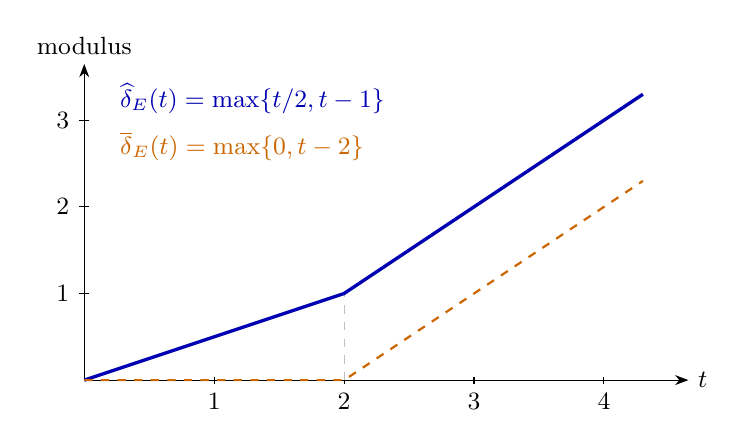
\begin{tikzpicture}[x=1.65cm,y=1.1cm,>=Stealth,font=\small]
 \draw[->] (0,0)--(4.65,0) node[right] {$t$};
 \draw[->] (0,0)--(0,3.65) node[above] {modulus};
 \foreach \x in {1,2,3,4} {
   \draw (\x,.04)--(\x,-.04) node[below] {$\x$};}
 \foreach \y in {1,2,3} {
   \draw (.04,\y)--(-.04,\y) node[left] {$\y$};}
 \draw[gray!50,dashed] (2,0)--(2,1);
 \draw[blue!70!black,very thick] (0,0)--(2,1)--(4.3,3.3);
 \draw[orange!80!black,thick,dashed] (0,0)--(2,0)--(4.3,2.3);
 \node[blue!70!black,anchor=west] at (.2,3.25)
   {$\whdelta_E(t)=\max\{t/2,t-1\}$};
 \node[orange!80!black,anchor=west] at (.2,2.7)
   {$\bardelta_E(t)=\max\{0,t-2\}$};
\end{tikzpicture}
\caption{The exact moduli of the original norm on $E$.
The averaged midpoint modulus is positive for every positive radius,
whereas the one-sided modulus vanishes through radius $2$.
Theorem~\ref{thm:exact} gives both equalities at each unit center.
These curves do not describe other equivalent norms.}
\label{fig:moduli}
\end{figure}


The existence of such spaces has an older history.  Bourgain and
Rosenthal constructed an $L^1$ subspace whose unit ball is relatively
compact in measure although the space fails the Radon--Nikodym property
\cite{BourgainRosenthal1980}.  Kadets and Werner refined its
finite-dimensional enlargement to obtain the Daugavet property
\cite[Lemma~2.4 and Theorem~2.5]{KW2004}. We give a complete realization of
their enlargement and limiting scheme in Section~\ref{kw:section}, so
the existence of an example and the calculation of its moduli form one
self-contained argument.

The two assumptions enter different parts of the proof.
In Section~\ref{sec:clips}, pointwise clipping at height $|x|/t$ turns the
measure-precompact ball into a norm-compact set.  Finitely many sign
functionals then force at least half the $L^1$ mass of every unit
direction in their common kernel to remain outside the clip, up to an
arbitrarily small error. This gives the lower
averaged bound.  Section~\ref{sec:weak-neighborhoods} develops the other
input: every weak neighborhood of a unit vector contains points almost
at distance two from it.  This is the needed case of Shvydkoy's
weak-open characterization of the Daugavet property
\cite[Lemma~3]{Shvydkoy2000}, obtained from the slice characterization
of Kadets, Shvidkoy, Sirotkin, and Werner \cite[Lemma~2.2]{KSSW2000}.
In Section~\ref{sec:curves}, correcting a finite-dimensional quotient
coordinate turns those almost diametral differences into directions in
any prescribed subspace of finite codimension, giving both upper curves.
Section~\ref{sec:renorming} uses the same weak-neighborhood
property at a near-maximizer of an arbitrary equivalent norm to rule
out AUC renorming. Section~\ref{kw:section} then constructs an increasing
sequence of finite-dimensional spaces whose closed union has both
required properties. At each step, multiplying selected old unit
vectors by independent positive variables creates new vectors almost
at distance two from every old unit vector, while averages of the new
vectors recover the selected ones. A uniform estimate places the
entire enlarged unit ball close in measure to the old ball. Summable
errors preserve total boundedness through the limit, and the averaging
property gives the Daugavet slice condition.

\section{Compact clips leave half the mass outside}\label{sec:clips}

In this section, $E$ is an infinite-dimensional closed real subspace of
a probability $L^1$ space, with its inherited norm. The clipping
argument uses only total boundedness of $B_E$ in measure.

For $x\in S_E$, $y\in E$, and $t>0$, the real scalar identity
$(|a+b|+|a-b|)/2=\max\{|a|,|b|\}$ gives
\begin{equation}\label{eq:overlap-identity}
 \frac{\|x+ty\|_1+\|x-ty\|_1}{2}-1
 =\int(t|y|-|x|)_+\,d\mathbb P
 =t\|y\|_1-\int\min\{|x|,t|y|\}\,d\mathbb P.
\end{equation}
Here $r_+=\max\{r,0\}$.  The lower bound therefore amounts to controlling
the overlap with $x$.

\begin{lemma}\label{lem:clips}
Let $E$ be an infinite-dimensional closed real subspace of
$L^1(\Omega,\mathbb P)$, where $\mathbb P$ is a probability measure.
If its unit ball $B_E$ is totally bounded in measure, then
$H_E(x,t)\ge\max\{t/2,t-1\}$ for every $x\in S_E$ and $t>0$.
\end{lemma}
\begin{proof}
Fix $x$ and $t$.  Clip a function $y$ at the pointwise height $|x|/t$:
\[
 C(y)=\operatorname{sgn}(y)\min\{|y|,|x|/t\}.
\]
The clipped functions need not belong to $E$.  Their norm closure
$K=\overline{C(B_E)}^{\,L^1}$ is compact.  Indeed, every sequence in $B_E$
has a subsequence Cauchy in measure.  Clipping is pointwise
$1$-Lipschitz, so the clipped subsequence is also Cauchy in measure.
For two of its terms $b_i,b_j$ and any $a>0$,
\[
 \|b_i-b_j\|_1
 \le a+\int_{\{|b_i-b_j|>a\}}2|x|/t\,d\mathbb P.
\]
Choose $a$ small, then use absolute continuity of the integral and the
measure-Cauchy property.  This proves that the subsequence is Cauchy in
$L^1$.  Completeness proves the compactness assertion.

Fix $\varepsilon>0$ and take a finite $\varepsilon$-net
$b_1,\ldots,b_m$ of $K$.  Set $\sigma_i=\operatorname{sgn}(b_i)$ and
\[
 F=\bigcap_{i=1}^m\ker\left(y\longmapsto
                 \int\sigma_i y\,d\mathbb P\right)\subseteq E.
\]
This is a closed subspace of finite codimension.  For $y\in S_F$, choose
$i$ with $\|C(y)-b_i\|_1<\varepsilon$.  Clipping preserves signs and
reduces absolute values, so
$\|y-C(y)\|_1=1-\|C(y)\|_1$.  Since $\int\sigma_i y=0$, we obtain
\[
 \|C(y)\|_1-\varepsilon
 \le\|b_i\|_1
 =\left|\int\sigma_i(b_i-y)\,d\mathbb P\right|
 \le1-\|C(y)\|_1+\varepsilon.
\]
Thus $\|C(y)\|_1\le1/2+\varepsilon$.
Equation~\eqref{eq:overlap-identity} now gives averaged increment at
least $t/2-t\varepsilon$ on $S_F$.  The same bound holds for
$\|y\|_1\ge1$ by radial monotonicity.  Taking the supremum over $F$ and
letting $\varepsilon\downarrow0$ gives $H_E(x,t)\ge t/2$.
The subspace is allowed to change with $\varepsilon$; this step does not
assert that one subspace attains the limiting bound.

For every $\|y\|_1\ge1$, the triangle inequality also gives
\[
 \frac{\|x+ty\|_1+\|x-ty\|_1}{2}-1\ge t\|y\|_1-1\ge t-1.
\]
Combining the two bounds proves the lemma.
\end{proof}

\begin{remark}[A separated-sequence proof]\label{rem:separated}
There is also a short contradiction argument giving the same half-mass
bound. Fix a unit center $x$, a radius $t>0$, and $0<a<1/2$.
Suppose no subspace of finite codimension had averaged increment at
least $at$ in every direction of norm at least one. By radial monotonicity and
Equation~\eqref{eq:overlap-identity}, every subspace of finite
codimension would then contain a unit vector $y$ with
$\|y-C(y)\|_1<a$. Inductively choose such $y_j$ in the kernels of
norm-one functionals norming the preceding vectors.  Then
$\|y_i-y_j\|_1\ge1$ for $i\ne j$.  Compactness of the clipped set gives
a subsequence whose clips are Cauchy in norm, whereas along this
subsequence
\[
 \|y_i-y_j\|_1
 \le\|y_i-C(y_i)\|_1+\|C(y_i)-C(y_j)\|_1
          +\|C(y_j)-y_j\|_1<2a+o(1)<1,
\]
a contradiction for sufficiently late pairs. Thus this argument yields
$H_E(x,t)\ge t/2$ by taking the supremum over the corresponding subspaces
and then letting $a\uparrow1/2$. The finite-net proof above identifies
an explicit finite family of functionals that removes the overlap.
\end{remark}

\section{Almost diametral points in weak neighborhoods}\label{sec:weak-neighborhoods}

To find almost diametral points subject to finitely many linear
constraints, we pass from slices to relatively weakly open subsets of
the ball. These points will supply both the upper bounds for the moduli
and the obstruction to AUC renorming. A \emph{slice} of $B_X$ is a nonempty set
\[
 H=\{y\in B_X:\ell(y)>\alpha\},\qquad
 \ell\in X^*,\quad\alpha\in\mathbb R.
\]
We first prove the geometric characterization of the Daugavet property
due to Kadets, Shvidkoy, Sirotkin, and Werner
\cite[Lemma~2.2]{KSSW2000}, also recalled by Kadets and Werner
\cite[Lemma~1.1]{KW2004}.

\begin{lemma}[Daugavet slice characterization]\label{lem:daugavet-slices}
A nonzero real Banach space $X$ has the Daugavet property if and only if,
for every $w\in S_X$, every $\rho>0$, and every slice $H$ of $B_X$,
there is $y\in H$ with $\|w+y\|\ge2-\rho$.
\end{lemma}
\begin{proof}
Suppose first that $X$ has the Daugavet property. If the functional
defining $H$ is zero, then $H=B_X$ and we may take $y=w$. Otherwise,
after dividing the functional and threshold by its norm, write
$H=\{y\in B_X:\ell(y)>\alpha\}$ with $\|\ell\|=1$ and $\alpha<1$.
Take $0<\eta<\min\{1-\alpha,\rho/2\}$. The rank-one operator
$Ty=\ell(y)w$ has norm one, so there is $y\in S_X$ with
$\|y+\ell(y)w\|>2-\eta$. Replacing $y$ by $-y$ if necessary makes
$\ell(y)\ge0$ without changing this inequality. It follows that
$\ell(y)>1-\eta>\alpha$ and
\[
 \|y+w\|\ge\|y+\ell(y)w\|-(1-\ell(y))>2-2\eta>2-\rho.
\]

Conversely, assume the slice condition and let
$Tz=\ell(z)v$ be a nonzero rank-one operator with $\|\ell\|=1$.
Set $a=\|v\|=\|T\|$ and $w=v/a$. For $0<\eta<1$, the slice condition
provides $y\in B_X$ with $\ell(y)>1-\eta$ and
$\|w+y\|\ge2-\eta$. A norm-one functional $\varphi$ norming $w+y$
takes value at least $1-\eta$ on each summand. Consequently,
\[
 \|I+T\|\ge\|y+Ty\|
 \ge\varphi(y)+a\ell(y)\varphi(w)
 \ge(1-\eta)+a(1-\eta)^2.
\]
Let $\eta\downarrow0$ and use $\|I+T\|\le1+\|T\|$.
The identity is immediate when $T=0$.
\end{proof}

The passage from slices to weak neighborhoods uses Bourgain's lemma
on convex combinations of slices
(see \cite{ANP2019} for the attribution).
We give a finite-dimensional proof.  Its use in passing to weak
neighborhoods follows the same pattern as Shvydkoy's proof of the
weak-open characterization \cite[Lemma~3]{Shvydkoy2000}.

\begin{lemma}[Bourgain's lemma]\label{lem:slice-combination}
Every nonempty relatively weakly open subset $U$ of a real Banach
space's closed unit ball contains a convex combination of nonempty
slices of that ball.
\end{lemma}
\begin{proof}
Choose $u\in U$, a continuous linear map $T:X\to\mathbb R^k$, and an
open set $O\subseteq\mathbb R^k$ such that
$u\in B_X\cap T^{-1}(O)\subseteq U$.  Put $D=\overline{T(B_X)}$.  We want to place a convex combination of
small slices of $D$ inside $O$ and then pull them back to $B_X$.
For this it suffices to approximate $T(u)$ by convex combinations of
exposed points, that is, unique maximizers of linear functionals on
$D$.  We first verify that $D$ is the closed convex hull of those points.
Put $M=\max_{q\in D}|q|$, using a Euclidean norm.  For a unit vector $a$
and $R>M$, choose $p_R\in D$ farthest from $-Ra$.  Expanding the squares
in $|q+Ra|\le|p_R+Ra|$ gives
\[
 2(p_R+Ra)\cdot(q-p_R)\le-|q-p_R|^2\qquad(q\in D).
\]
Thus $p_R$ is the unique maximizer of the linear functional with
coefficient $p_R+Ra$.  If $q_a$ maximizes $a\cdot q$ on $D$, the same
comparison gives
\[
 0\le a\cdot q_a-a\cdot p_R
 \le\frac{|p_R|^2-|q_a|^2}{2R}\le\frac{M^2}{2R}.
\]
The exposed points therefore have the same supremum as $D$ for every
linear functional.  Separation proves the closed-convex-hull assertion,
also when $D$ is a singleton.

Since $T(u)\in O$, there are exposed points $p_1,\ldots,p_l$ and
positive weights $\lambda_i$ summing to one such that
$p=\sum_i\lambda_i p_i\in O$.  Choose $r>0$ with the Euclidean ball
$B(p,r)\subseteq O$.  If $a_i\cdot q$ exposes $p_i$, compactness and
uniqueness of its maximum give a threshold $\beta_i<a_i\cdot p_i$ with
\[
 \{q\in D:a_i\cdot q>\beta_i\}\subseteq B(p_i,r).
\]
The sets $H_i=\{y\in B_X:a_i\cdot T(y)>\beta_i\}$ are nonempty slices,
since $T(B_X)$ is dense in $D$.  For $y_i\in H_i$,
\[
 \left|T\left(\sum_i\lambda_i y_i\right)-p\right|
 \le\sum_i\lambda_i|T(y_i)-p_i|<r.
\]
Their convex combination consequently belongs to $U$.
\end{proof}

The slice property can now be applied successively within the slices
provided by Bourgain's lemma.  This gives the following specialization
of Shvydkoy's weak-open result \cite[Lemma~3]{Shvydkoy2000}.

\begin{lemma}\label{lem:diametral}
If $X$ has the Daugavet slice property, then, for every $x\in S_X$ and
every relatively weakly open neighborhood $U$ of $x$ in $B_X$,
\[
 \sup_{v\in U}\|v-x\|=2.
\]
\end{lemma}
\begin{proof}
By Lemma~\ref{lem:slice-combination}, choose slices $H_i$ and positive
weights $\lambda_i$ such that $\sum_i\lambda_i=1$ and
$\sum_i\lambda_iH_i\subseteq U$.  Fix $0<\eta<1$ and set $z_0=-x$.
At step $i$, apply the slice property at $z_{i-1}/\|z_{i-1}\|$ to choose
$y_i\in H_i$ with
$\|z_{i-1}/\|z_{i-1}\|+y_i\|\ge2-\eta$.
A norm-one functional norming this sum takes value at least $1-\eta$
on each of its two summands.  Therefore, with
$z_i=z_{i-1}+\lambda_i y_i$,
\[
 \|z_i\|\ge(1-\eta)(\|z_{i-1}\|+\lambda_i)>0.
\]
The induction is well defined and yields
\[
 \|z_l\|\ge(1-\eta)^l+
    \sum_{i=1}^l\lambda_i(1-\eta)^{l-i+1}
 \ge2(1-\eta)^l.
\]
Now $v=\sum_i\lambda_i y_i\in U$ and $z_l=v-x$.  Let
$\eta\downarrow0$; the reverse bound follows from $v,x\in B_X$.
\end{proof}

\section{One family of directions gives both curves}\label{sec:curves}

\begin{proof}[Proof of the formulas in Theorem~\ref{thm:exact}]
Lemma~\ref{lem:clips} gives the averaged lower bound.  For the one-sided
bound, choose a norm-one functional $\varphi$ with
$\varphi(x)=1$.  Every $y\in S_{\ker\varphi}$ satisfies
\[
 \|x+ty\|\ge1,\qquad \|x+ty\|\ge t-1.
\]
Hence $D_E(x,t)\ge\max\{0,t-2\}$.

For the upper bounds, fix any $F\in\operatorname{cof}(E)$ and choose a
bounded finite-rank projection $P$ with kernel $F$.  Such a projection
is obtained by composing the quotient map with a linear section of
$E/F$.  For $0<\varepsilon<1/2$,
\[
 U_\varepsilon=\{v\in B_E:\|P(v-x)\|<\varepsilon\}
\]
is a relatively weakly open neighborhood of $x$.  The finite-dimensional
range of $P$ makes it weak-to-norm continuous.  By
Lemma~\ref{lem:diametral}, choose $v_\varepsilon\in U_\varepsilon$ with
$\|v_\varepsilon-x\|>2-\varepsilon$, and put
\[
 z_\varepsilon=(I-P)(v_\varepsilon-x),\quad
 L_\varepsilon=\|z_\varepsilon\|,\quad
 y_\varepsilon=z_\varepsilon/L_\varepsilon\in S_F.
\]
Then
\[
 2-2\varepsilon<L_\varepsilon\le2+\varepsilon,
 \qquad \|x+z_\varepsilon\|\le1+\varepsilon.
\]
Thus the directions lie exactly in $F$, their unnormalized lengths tend
to two, and the translated endpoints remain close to $B_E$.

For any $t>0$, set $\lambda=\min\{t/L_\varepsilon,1\}$.  The identity
\[
 x+t y_\varepsilon
 =(1-\lambda)x+\lambda(x+z_\varepsilon)
       +(t-L_\varepsilon)_+y_\varepsilon
\]
and the triangle inequality give the single bound
\[
 \|x+t y_\varepsilon\|
 \le1+\varepsilon+(t-L_\varepsilon)_+.
\]
The right-hand side converges to $1+(t-2)_+=\max\{1,t-1\}$.  Since
$\|x-t y_\varepsilon\|\le1+t$, the one-sided and averaged increments
have upper limits at most
\[
 (t-2)_+,\qquad \frac{t+(t-2)_+}{2},
\]
respectively.  These are $\max\{0,t-2\}$ and
$\max\{t/2,t-1\}$.  In particular the argument includes $t=2$, where
the two branches meet.  Each inner infimum for the fixed $F$ is at most
the corresponding limit.  Taking the supremum over $F$ proves the
upper bounds.  Both formulas hold for every unit center, so taking the
infimum over centers leaves them unchanged.
\end{proof}

\section{Why a different norm cannot be AUC}\label{sec:renorming}

The one-sided modulus vanishes for $0<t\le2$, so the inherited norm is not AUC.
Ruling out all equivalent norms requires the weak-neighborhood
property itself. The following argument applies to any infinite-dimensional
real Banach space in which every relatively weakly open neighborhood of a unit
vector contains points of the unit ball arbitrarily close to distance
two from that vector, as in Lemma~\ref{lem:diametral}.

\begin{proof}[Proof of the renorming assertion in Theorem~\ref{thm:exact}]
Suppose $N$ is an equivalent AUC norm.  Choose $a>0$ with
$N(u)\ge a\|u\|$ for all $u$, and put
$R=\sup_{u\in B_E}N(u)<\infty$.  Fix, in this order,
\[
 t_0=\frac{a}{4R},\qquad
 0<\gamma<\overline\delta_N(t_0),\qquad
 x_0\in S_E\ \text{with}\ (1+\gamma)N(x_0)>R.
\]
The last choice is possible since $R=\sup_{u\in S_E}N(u)$.
The definition of $\overline\delta_N(t_0)$ at $x_0/N(x_0)$ supplies
$F\in\operatorname{cof}(E)$ such that
\begin{equation}\label{eq:auc-outside}
 N(x_0+z)\ge(1+\gamma)N(x_0)
 \quad\text{if }z\in F,\quad N(z)\ge t_0N(x_0).
\end{equation}
To justify the entire range of radii, convexity gives, for $N(w)=1$ and
$r\ge t_0$,
\[
 N(x_0/N(x_0)+rw)-1
 \ge\frac r{t_0}\bigl(N(x_0/N(x_0)+t_0w)-1\bigr).
\]

Choose
$0<\eta<\min\{(1+\gamma)N(x_0)-R,a/4\}$.  The set
\[
 U=\{u\in B_E:\inf_{z\in F}N(u-x_0-z)<\eta\}
\]
is a relatively weakly open neighborhood of $x_0$: the infimum is the
norm in the finite-dimensional quotient $E/F$.  Equivalent norms have
the same continuous functionals, hence the same weak topology.
For $u\in U$, choose $z\in F$ with $N(u-x_0-z)<\eta$.
If $N(z)\ge t_0N(x_0)$, Equation~\eqref{eq:auc-outside} gives
\[
 N(u)>(1+\gamma)N(x_0)-\eta>R,
\]
contrary to $u\in B_E$.  Thus
\[
 N(u-x_0)<t_0N(x_0)+\eta\le t_0R+\eta<a/2,
 \qquad\|u-x_0\|<1/2.
\]
This contradicts Lemma~\ref{lem:diametral}.
\end{proof}

\section{Constructing the measure-precompact Daugavet space}
\label{kw:section}

The preceding results apply to a space with two rather different
properties: its unit ball is small for convergence in measure, while
its slices contain vectors almost at distance two from any prescribed
unit vector.
We now construct such a space.  The construction is due to
Kadets and Werner \cite[Lemma~2.4 and Theorem~2.5]{KW2004}, who refine
the method of Bourgain and Rosenthal \cite{BourgainRosenthal1980}.
We give all the estimates needed for the finite-dimensional enlargement
and its iteration. The explicit multipliers below and the constants
$10$, $54$, and $108$ belong to the quantitative realization given here;
the enlargement and iteration scheme is the credited construction.

The idea is to multiply an old unit vector by a positive random variable
which has mean one but is small with high probability.  Each product has
small $L^1$ overlap with every old unit vector, so the norm of their sum is
almost two.  Averaging sufficiently many products recovers the old vector
in norm.  The main additional task is to control every vector in the
new unit ball, which permits the iteration to preserve precompactness
in measure.

Throughout this section,
\[
 (\Omega,\PP)=([0,1]^{\N},\lambda^{\N}),
 \qquad L^1=L^1(\Omega,\PP;\R),
\]
and $\norm{\cdot}$ denotes the $L^1$ norm.  Write $B(G)$ and $S(G)$ for
the closed unit ball and unit sphere of a subspace $G$.  A space depends
on finitely many coordinates if one common finite set of coordinates
determines all its elements.

Recall the metric from \eqref{eq:measure-metric}, on measurable functions
modulo equality almost everywhere:
\begin{equation}\label{kw:metric}
 d(f,g)=\inf\{a>0:\PP(\abs{f-g}>a)<a\}.
\end{equation}
This metric induces convergence in measure.  For example, if
$\PP(\abs{f-g}>a)<a$ and $\PP(\abs{g-h}>b)<b$, the union bound gives
$\PP(\abs{f-h}>a+b)<a+b$; taking infima proves the triangle inequality.
The identity $d(f,g)=0$ is equivalent to $f=g$ almost everywhere, and
the convergence assertion follows directly from the thresholds in
\eqref{kw:metric}.  Markov's inequality also gives
$d(f,g)\le\norm{f-g}^{1/2}$, so norm convergence implies convergence
for $d$.

\begin{theorem}[Kadets--Werner construction]\label{kw:existence}
There is an infinite-dimensional closed real subspace $E\subseteq L^1$
such that $B(E)$ is totally bounded for $d$ and has the following slice
property: for every $w\in S(E)$, every nonempty slice
\[
 H=\{y\in B(E):\ell(y)>\alpha\},\qquad \ell\in E^*,\quad\alpha\in\R,
\]
and every $\rho>0$, there is $y\in H\cap S(E)$ such that
$\norm{w+y}\ge2-\rho$.  In particular, $E$ has the Daugavet property.
\end{theorem}

\subsection{The finite-dimensional enlargement}

We need the new unit vectors to be almost additive in norm with every
old unit vector, and their averages to approximate selected old vectors.
The third conclusion below keeps the entire new unit ball close, in
measure, to the old unit ball.

\begin{lemma}\label{kw:enlargement}
Suppose $G\ne\{0\}$ is a finite-dimensional subspace of $L^1$ depending
on finitely many coordinates, $m\ge1$, $u_1,\dots,u_m\in S(G)$, and $0<h<1$.
There are a finite-dimensional $G'\supseteq G$ depending on finitely
many coordinates, an integer $n\ge1$, and vectors
$v_{kj}\in S(G')$ $(1\le k\le m,\ 1\le j\le n)$ such that
\begin{align}
 \norm{w+v_{kj}}&\ge2-h
 &&(w\in S(G),\ k\le m,\ j\le n),\label{kw:enlarge-a}\\
 \norm{u_k-\frac1n\sum_{j=1}^n v_{kj}}&\le h
 &&(k\le m),\label{kw:enlarge-b}\\
 \text{for every }g\in B(G')\text{ there is }\psi_0\in B(G)
 &\text{ with }d(g,\psi_0)\le h.\label{kw:enlarge-c}
\end{align}
\end{lemma}

To prove the lemma, we will use independent positive multipliers whose
mean is one and whose mass is concentrated near zero.  The next estimate
controls their linear combinations; this is what the whole-ball
conclusion requires beyond control of the selected vectors themselves.

\subsection{A heavy-tail estimate}

The following variable has mean one for every $p>1$, although it converges
to zero in probability as $p\downarrow1$.  The estimate for differences
will control arbitrary linear combinations in an enlarged unit ball.

\begin{lemma}\label{kw:heavy-tail}
Let $1<p\le3/2$, $s=(p-1)/p$, and $f=sV^{-1/p}$, where $V$ is uniform
on $(0,1)$.  Let $Y_1,\dots,Y_n$ be independent variables, each distributed
as the difference of two independent copies of $f$.  For real scalars
$a_1,\dots,a_n$, put
$A=(\sum_{j=1}^n\abs{a_j}^{p})^{1/p}$ and $Z=\sum_{j=1}^n a_jY_j$.
Then $\E f=1$ and
\begin{equation}\label{kw:heavy-bounds}
 \PP(\abs Z>u)\le10(sA/u)^p\quad(u>0),
 \qquad \E\abs Z\ge A/54.
\end{equation}
\end{lemma}

The lower estimate bounds $A$ from an $L^1$ bound on $Z$;
the upper estimate then gives concentration in probability uniformly in $n$.

\begin{proof}
Direct integration gives $\E f=sp/(p-1)=1$, and
$\PP(f>u)=(s/u)^p$ for $u\ge s$.  For all $u>0$ the same expression
is an upper bound.  If $Y=f-f'$ for independent copies, then $Y$ is
symmetric and $\PP(\abs Y>u)\le2(s/u)^p$.
For fixed $u>0$, the variables
$X_j=a_jY_j\mathbf1_{\{\abs{a_jY_j}\le u\}}$ are independent and
centered, and
\[
 \E X_j^2
 \le\int_0^u 2v\,\PP(\abs{a_jY_j}>v)\,dv
 \le\frac{4(s\abs{a_j})^p u^{2-p}}{2-p}.
\]
Except on the event that some $\abs{a_jY_j}>u$, the sums $Z$ and
$\sum_jX_j$ agree.  The union bound and Chebyshev's inequality therefore
give
\[
 \PP(\abs Z>u)
 \le\left(2+\frac4{2-p}\right)(sA/u)^p
 \le10(sA/u)^p.
\]

For the lower bound, when $u\ge s$, the event
$\{f>u+2s,\ f'\le2s\}$ gives
\[
 \PP(\abs Y>u)
 \ge\left(\frac{s}{u+2s}\right)^p(1-2^{-p})
 \ge\frac1{18}(s/u)^p.
\]
Here $u+2s\le3u$, $1-2^{-p}\ge1/2$, and $3^p\le9$.
Suppose $A>0$ and omit zero coefficients.  Since $\abs{a_j}\le A$,
independence implies, for $u\ge sA$,
\begin{align*}
 \PP\left(\max_j\abs{a_jY_j}>u\right)
 &\ge1-\exp\left(-\frac1{18}(sA/u)^p\right)\\
 &\ge\frac1{36}(sA/u)^p.
\end{align*}
The last inequality uses $1-e^{-v}\ge v/2$ for $0\le v\le1$.
Adjoin independent signs $\varepsilon_j\in\{-1,1\}$ of equal probability.
For each fixed realization of the terms, averaging first over the sign
of a term of largest absolute value gives
\[
 \E_{\varepsilon}\abs{\sum_j\varepsilon_j a_jY_j}
 \ge\max_j\abs{a_jY_j},
\]
because $(\abs{b+c}+\abs{b-c})/2\ge\abs c$.
The signed sum has the same law as $Z$, by independence and symmetry.
Consequently,
\[
 \E\abs Z\ge\E\max_j\abs{a_jY_j}
 \ge\frac1{36}\int_{sA}^\infty(sA/u)^p\,du
 =\frac{A}{36p}\ge\frac A{54}.
\]
If $A=0$, both assertions are immediate.
\end{proof}

\subsection{Proof of the enlargement}

The scalar estimates now let us control all linear combinations in the
new space.  We prove the three conclusions of Lemma~\ref{kw:enlargement}
in the order that permits the number of multipliers to be chosen last.

\begin{proof}[Proof of Lemma~\ref{kw:enlargement}]
We first fix the distribution of the new multipliers and prove the first
and third conclusions uniformly in their number.  Only then will we
choose the number of multipliers to obtain the averaging conclusion.

\emph{Parameter choices.}
Choose $c\in(0,h/4)$, and then $r,q>0$ sufficiently small that
\begin{equation}\label{kw:rq-choice}
 mq<1,\qquad
 mq+h^{-1}\bigl(2mr+(1-mq)^{-1}-1\bigr)<h.
\end{equation}
With $s=(p-1)/p$, choose $1<p\le3/2$ close enough to $1$ that
\begin{equation}\label{kw:p-choice}
 s<c,\qquad 2\bigl((s/c)^p+c\bigr)<h,
 \qquad 10(108s/r)^p<q.
\end{equation}
These choices are possible because $s\to0$ as $p\downarrow1$.
We fix $p$ now; the integer $n$ will be chosen last.

\emph{Near-additivity with the old space.}
For any prospective $n$, take $mn$ independent copies $f_{kj}$ of the
variable $f$ in Lemma~\ref{kw:heavy-tail}, each on a fresh coordinate,
and put
\[
 v_{kj}=u_kf_{kj},\qquad
 G'_n=\operatorname{span}\bigl(G\cup\{v_{kj}:k\le m,\ j\le n\}\bigr).
\]
Independence from the old coordinates gives $\norm{v_{kj}}=1$.
For every $w\in S(G)$,
\begin{align*}
 \norm{w+v_{kj}}
 &\ge2-2\E\min(\abs w,\abs{u_k}f_{kj})\\
 &\ge2-2\bigl(\PP(f>c)+c\bigr)>2-h.
\end{align*}
Indeed, on $\{f_{kj}>c\}$ bound the minimum by $\abs w$, and on its
complement by $c\abs{u_k}$; independence then gives the last bound.
Thus \eqref{kw:enlarge-a} holds for every $n$.

\emph{Approximation of the whole unit ball.}
We next prove \eqref{kw:enlarge-c}, also uniformly in $n$.
Fix $g\in B(G'_n)$ and choose any representation
\[
 g=x+\sum_{k=1}^m u_kz_k,\qquad
 x\in G,\quad z_k=\sum_{j=1}^n a_{kj}f_{kj}.
\]
Fix $k$.  On an auxiliary product probability space resample all the
variables in the $k$th group, leaving the old coordinates and all other
groups unchanged.  Write $z'_k$ for the resampled sum and $g^{(k)}$
for the resulting function.  The new variables are independent copies,
so $g^{(k)}$ has the same law as $g$, and
\[
 \E\abs{z_k-z'_k}
 =\E\abs{u_k(z_k-z'_k)}
 =\E\abs{g-g^{(k)}}\le2.
\]
The first equality uses $\norm{u_k}=1$ and independence of the old
coordinates.  Lemma~\ref{kw:heavy-tail}, applied to the differences of
the paired copies, therefore gives
\begin{equation}\label{kw:coefficient-bound}
 A_k=\left(\sum_j\abs{a_{kj}}^p\right)^{1/p}\le108,
 \qquad
 \PP(\abs{z_k-z'_k}>r)\le10(108s/r)^p<q.
\end{equation}
In particular, the bound does not depend on $n$ or on the chosen
representation of $g$.

The estimate for $z_k-z'_k$ says that $z_k$ is concentrated near some
constant.  Indeed, averaging the conditional probability over $z'_k$
gives a deterministic $c_k\in\R$ with
$\PP(\abs{z_k-c_k}>r)<q$.
These constants may depend on $g$; no simultaneous choice is needed.
Set
\[
 \psi=x+\sum_{k=1}^m c_ku_k\in G,
 \qquad D=\bigcap_{k=1}^m\{\abs{z_k-c_k}\le r\}.
\]
The event $D$ depends only on the fresh coordinates, has probability
at least $1-mq$, and on $D$ we have
$\abs{g-\psi}\le r\sum_k\abs{u_k}$.
Its independence from the old coordinates gives
\[
 1\ge\E(\abs g\mathbf1_D)
 \ge\PP(D)(\norm\psi-mr),
 \qquad \norm\psi\le mr+(1-mq)^{-1}.
\]
At this point $\psi$ need not belong to the old unit ball.  Set
$\psi_0=\psi/\max\{1,\norm\psi\}\in B(G)$.  The cost of this normalization
is bounded by
\[
 \norm{\psi-\psi_0}
 \le mr+(1-mq)^{-1}-1.
\]
Markov's inequality restricted to $D$ and the bound on its complement
now yield
\begin{align*}
 \PP(\abs{g-\psi_0}>h)
 &\le mq+h^{-1}\bigl(mr+\norm{\psi-\psi_0}\bigr)\\
 &\le mq+h^{-1}\bigl(2mr+(1-mq)^{-1}-1\bigr)<h.
\end{align*}
This proves \eqref{kw:enlarge-c} for every $n$.

We have now proved both near-additivity and whole-ball approximation
without placing an upper bound on $n$.

\emph{Recovering the old vectors by averages.}
It remains to choose $n$ for \eqref{kw:enlarge-b}.
For independent copies $f_1,\dots,f_n$ of the fixed integrable variable
$f$, write $f^M=\min\{f,M\}$.  Truncating, centering, and applying the
variance bound to the bounded independent copies gives
\begin{equation}\label{kw:lln}
 \E\abs{\frac1n\sum_{j=1}^nf_j-1}
 \le2\E(f-f^M)+\sqrt{\operatorname{Var}(f^M)/n}.
\end{equation}
The first term tends to zero as $M\to\infty$; after $M$ is fixed the
second tends to zero as $n\to\infty$.  Choose $n$ so that the left side
is at most $h$.  All groups have the same law, and independence gives
\[
 \norm{u_k-\frac1n\sum_jv_{kj}}
 =\E\abs{1-\frac1n\sum_jf_{kj}}\le h
 \qquad(k\le m).
\]
Taking $G'=G'_n$ completes the proof.  This space uses just finitely many
additional coordinates; the earlier two conclusions persist because
their estimates held for every finite $n$.
\end{proof}

\subsection{Passage to the closed space}

We apply the enlargement to finer and finer nets of the old unit sphere.
The summable errors keep the eventual unit ball precompact in measure;
the approximation by averages ensures that every slice eventually
contains one of the new unit vectors.

\begin{proof}[Proof of Theorem~\ref{kw:existence}]
Start with $G_1=\operatorname{span}\{1\}$ and put $h_b=2^{-b}$.
Given $G_b$, choose a finite $h_b$-net
$\{u_{b,k}:1\le k\le m_b\}$ of $S(G_b)$ in norm and apply
Lemma~\ref{kw:enlargement} with $h=h_b$.  Denote the resulting space by
$G_{b+1}$ and its new unit vectors by $v_{b,kj}$, $1\le j\le n_b$.
All stages depend on finitely many coordinates, so the construction
continues on $\Omega$.  Set
\[
 E=\overline{\bigcup_{b\ge1}G_b}^{\,\norm{\cdot}}\subseteq L^1.
\]
Each inclusion $G_b\subseteq G_{b+1}$ is strict: if any $v_{b,kj}$
belonged to $G_b$, substituting $w=-v_{b,kj}$ in
\eqref{kw:enlarge-a} would give $0\ge2-h_b$.
Thus $E$ is infinite-dimensional.

\emph{The entire unit ball is totally bounded in measure.}
The union
$\bigcup_bB(G_b)$ is norm dense in $B(E)$: if $x_j$ in the algebraic
union tends to $x\in B(E)$, then
$x_j/\max\{1,\norm{x_j}\}$ also tends to $x$.
Repeated use of \eqref{kw:enlarge-c} gives, for $a>b$ and $g\in B(G_a)$,
\[
 \inf_{\psi\in B(G_b)}d(g,\psi)
 \le\sum_{l=b}^{a-1}h_l
 \le\sum_{l=b}^\infty h_l=2^{1-b}.
\]
The bound is automatic for $a\le b$.  Distance to a fixed nonempty
set is a $1$-Lipschitz function for $d$, so norm density and
\eqref{kw:metric} extend it to every $g\in B(E)$.
The set $B(G_b)$ is norm compact and therefore $d$-compact.
Given $\eps>0$, choose $b$ with $2^{1-b}<\eps/2$ and a finite
$\eps/2$-net of $B(G_b)$ for $d$.  The preceding distance estimate
shows that this is an $\eps$-net of $B(E)$.

\emph{The Daugavet slice property.}
Now fix $w,H,\ell,\alpha,\rho$ as in Theorem~\ref{kw:existence}.
There is $u\in S(E)$ with $\ell(u)>\alpha$: the supremum of a linear
functional over the ball equals its supremum over the sphere, including
when the functional is zero.  Normalizing approximants from the
increasing union gives $u^{(b)},w^{(b)}\in S(G_b)$ with
$u^{(b)}\to u$ and $w^{(b)}\to w$ in norm.
Choose a net point $u_{b,k_b}$ with
$\norm{u_{b,k_b}-u^{(b)}}\le h_b$ and set
\[
 a_b=\frac1{n_b}\sum_{j=1}^{n_b}v_{b,k_bj}.
\]
By \eqref{kw:enlarge-b},
$\norm{a_b-u}\le2h_b+\norm{u^{(b)}-u}\to0$.
Thus $\ell(a_b)>\alpha$ for all sufficiently large $b$, and for each
such $b$ at least one summand $v_{b,k_bj}$ lies in $H$.
For every summand, \eqref{kw:enlarge-a} also gives
\[
 \norm{w+v_{b,k_bj}}
 \ge2-h_b-\norm{w-w^{(b)}}.
\]
Take $b$ large enough that the last two error terms sum to less than
$\rho$.  The summand in $H$ is the required unit vector.

Finally, Lemma~\ref{lem:daugavet-slices} turns this slice property into
$\norm{I+T}=1+\norm T$ for every rank-one operator $T$ on $E$.
\end{proof}

\bibliographystyle{plainnat}
\bibliography{references}
\end{document}
